\section*{Appendice}
\addcontentsline{toc}{section}{Appendice}

\begin{figure}[H]
    \centering
    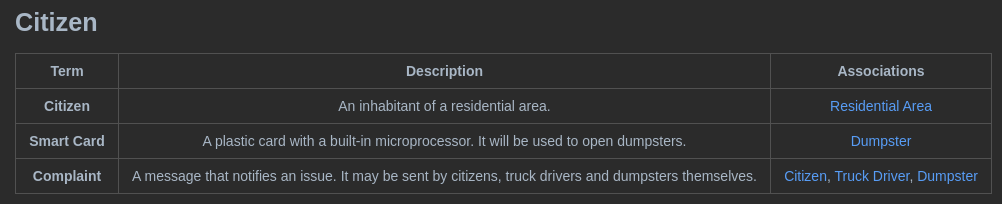
\includegraphics[width=\textwidth]{img/citizen-ubiquitous-language}
    \caption{\textit{Ubiquitous Language}: i termini del topic "cittadino".}
    \label{fig:img/citizen-ubiquitous-language}
\end{figure}


\begin{figure}[H]
    \centering
    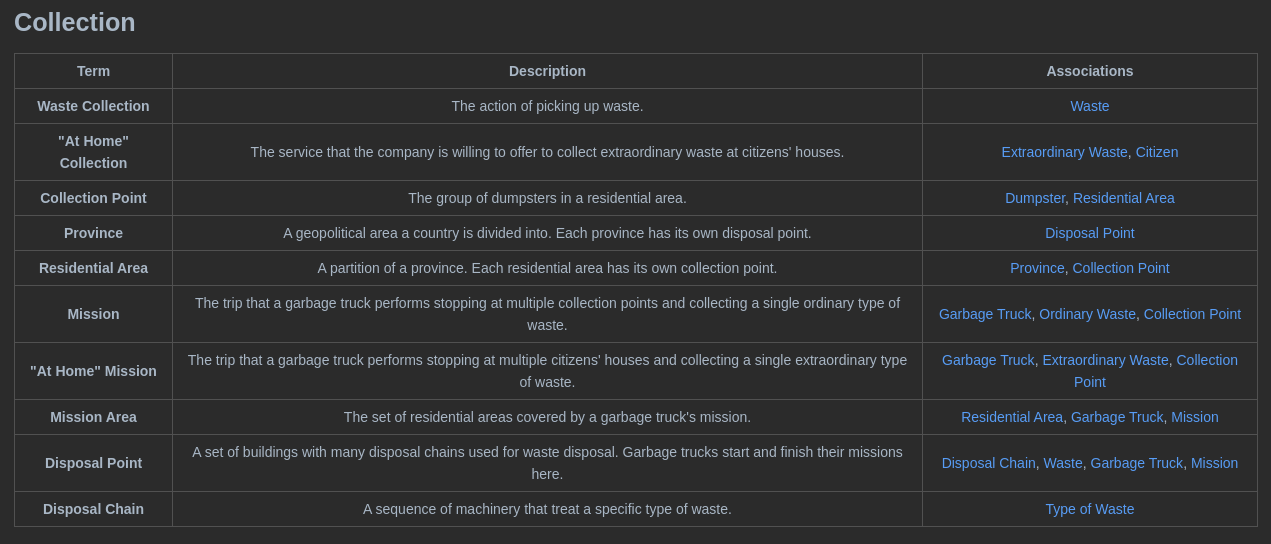
\includegraphics[width=\textwidth]{img/collection-ubiquitous-language}
    \caption{\textit{Ubiquitous Language}: i termini del topic "raccolta".}
    \label{fig:img/collection-ubiquitous-language}
\end{figure}


\begin{figure}[H]
    \centering
    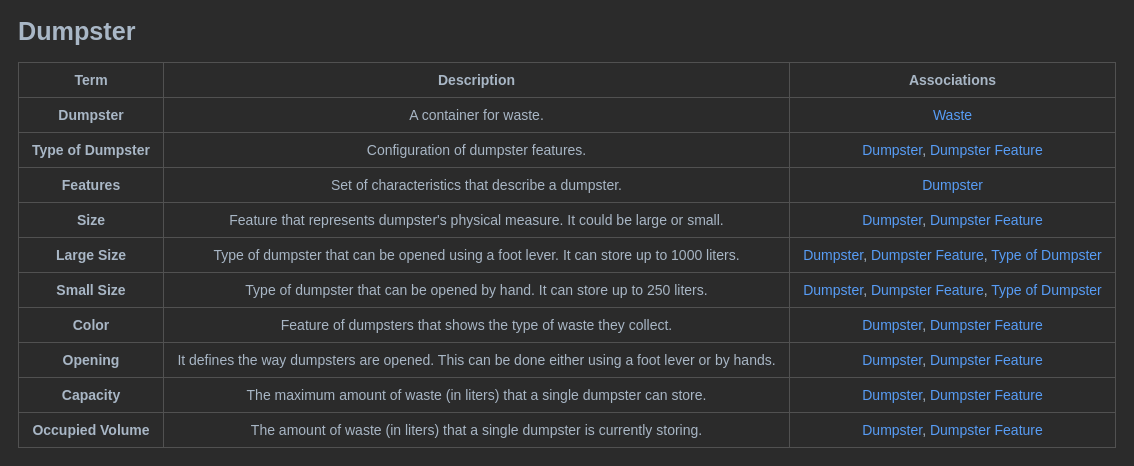
\includegraphics[width=\textwidth]{img/dumpster-ubiquitous-language}
    \caption{\textit{Ubiquitous Language}: i termini del topic "cassonetti".}
    \label{fig:img/dumpster-ubiquitous-language}
\end{figure}


\begin{figure}[H]
    \centering
    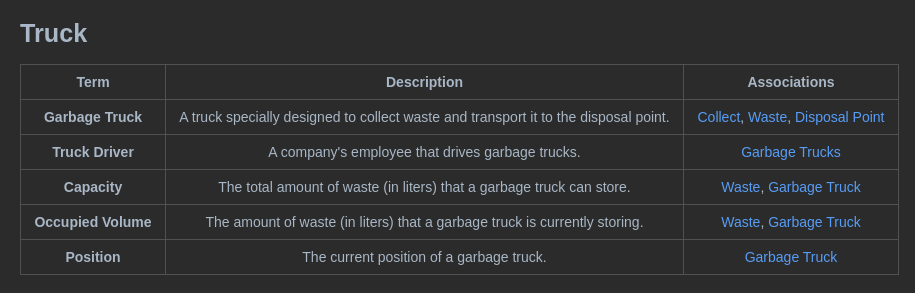
\includegraphics[width=\textwidth]{img/truck-ubiquitous-language}
    \caption{\textit{Ubiquitous Language}: i termini del topic "camioncini".}
    \label{fig:img/truck-ubiquitous-language}
\end{figure}


\begin{figure}[H]
    \centering
    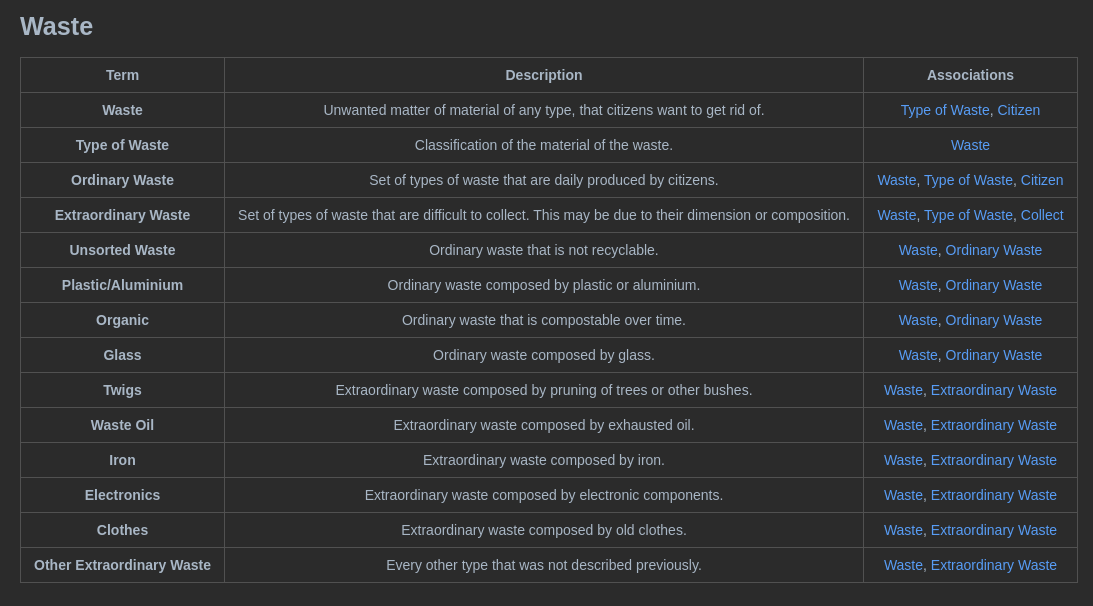
\includegraphics[width=\textwidth]{img/waste-ubiquitous-language}
    \caption{\textit{Ubiquitous Language}: i termini del topic "rifiuti".}
    \label{fig:img/waste-ubiquitous-language}
\end{figure}


\begin{figure}[H]
    \centering
    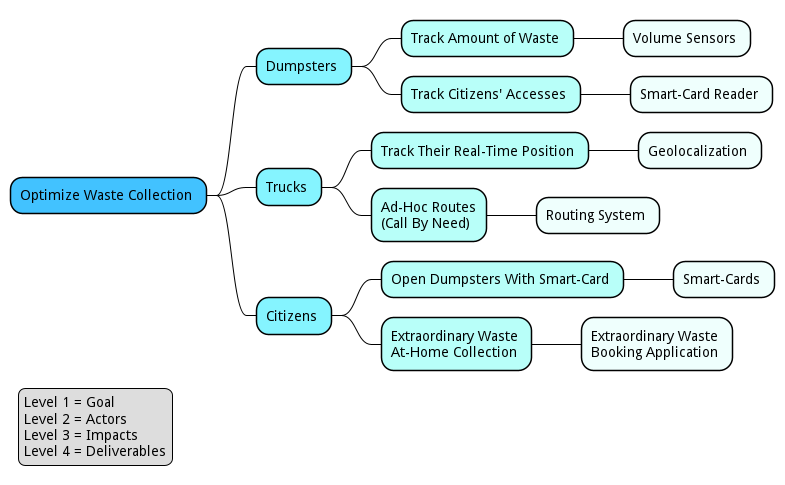
\includegraphics[width=\textwidth]{uml/impact-mapping.pm}
    \caption{\textit{Impact map} che, a partire dal \textit{goal}, mostra quali sono le soluzioni con maggiore impatto sugli attori del sistema.}
    \label{fig:uml/impact-mapping}
\end{figure}


\begin{figure}[H]
    \centering
    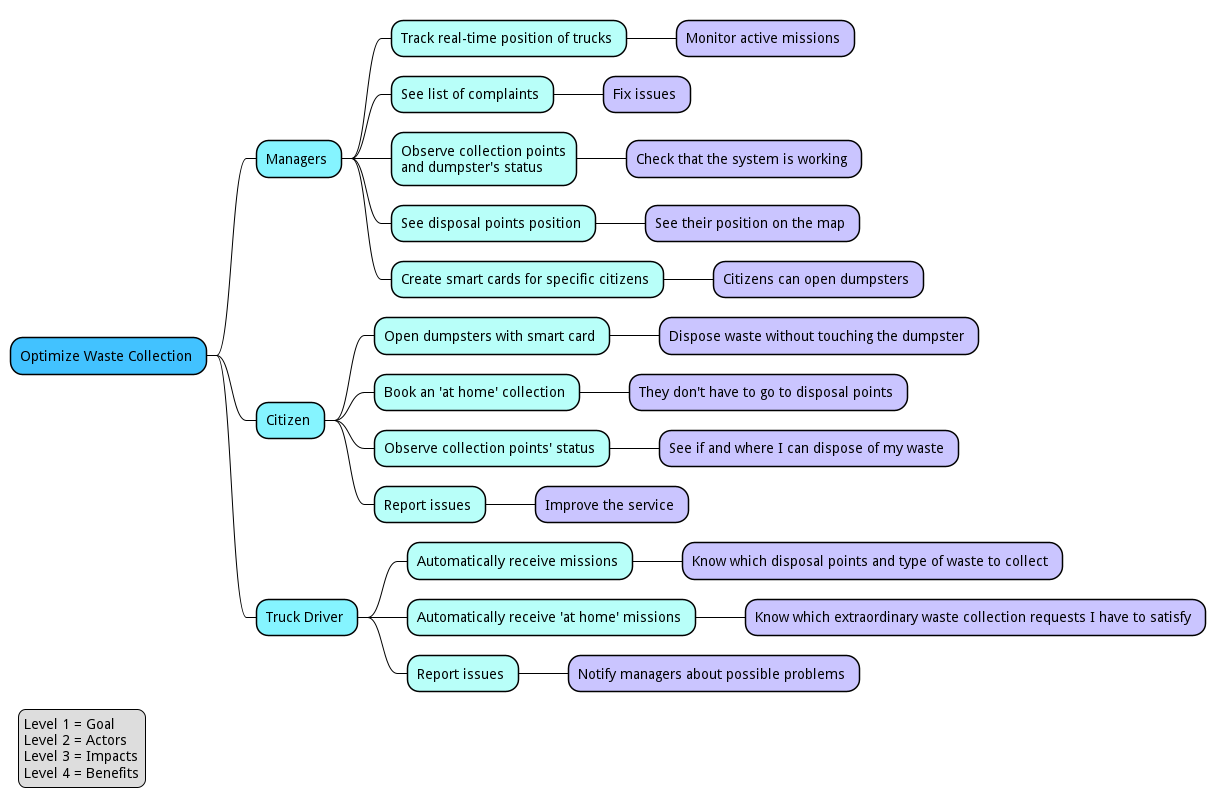
\includegraphics[width=\textwidth]{uml/benefit-mapping.pm}
    \caption{\textit{Impact map} che, a partire dal \textit{goal}, mostra chi sono gli attori che beneficiano maggiormente dai cambiamenti introdotti dal sistema.}
    \label{fig:uml/benefit-mapping}
\end{figure}


\begin{figure}[H]
    \centering
    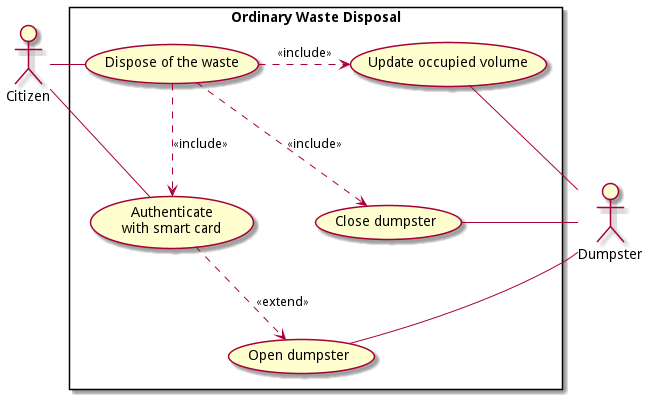
\includegraphics[width=\textwidth]{uml/ordinary-disposal-use-cases.pm}
    \caption{Diagramma dei casi d'uso dello scenario del conferimento di rifiuti ordinari.}
    \label{fig:uml/ordinary-disposal-use-cases}
\end{figure}


\begin{figure}[H]
    \centering
    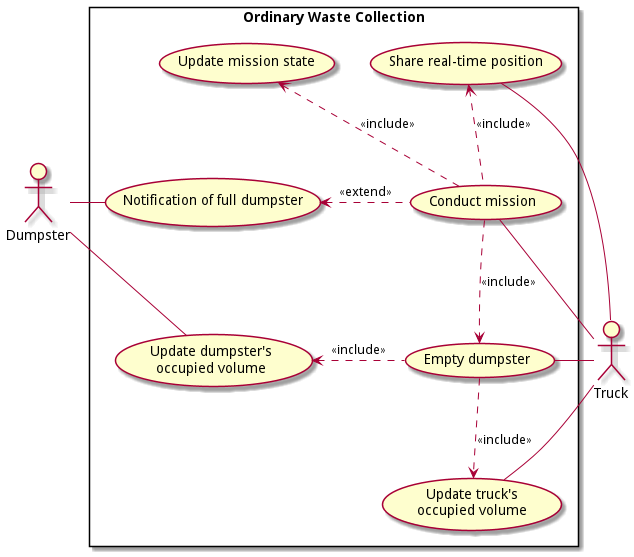
\includegraphics[width=\textwidth]{uml/ordinary-collection-use-cases.pm}
    \caption{Diagramma dei casi d'uso dello scenario della raccolta di rifiuti ordinari.}
    \label{fig:uml/ordinary-collection-use-cases}
\end{figure}


\begin{figure}[H]
    \centering
    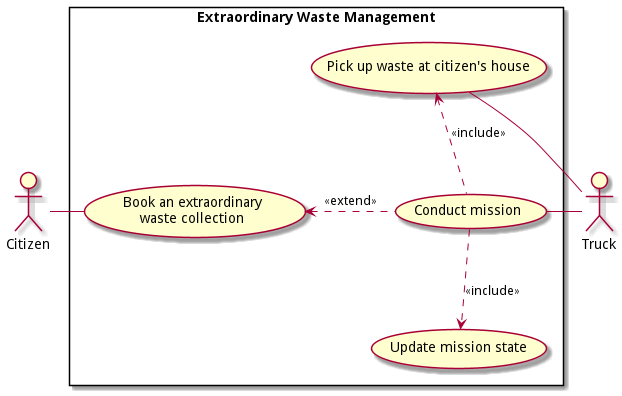
\includegraphics[width=\textwidth]{uml/extraordinary-management-use-cases.pm}
    \caption{Diagramma dei casi d'uso dello scenario della gestione di rifiuti straordinari.}
    \label{fig:uml/extraordinary-management-use-cases}
\end{figure}


\begin{figure}[H]
    \centering
    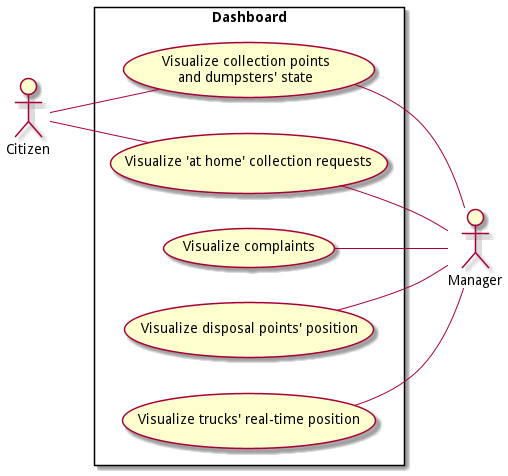
\includegraphics[width=\textwidth]{uml/dashboard-use-cases.pm}
    \caption{Diagramma dei casi d'uso dello scenario dell'utilizzo della dashboard.}
    \label{fig:uml/dashboard-use-cases}
\end{figure}


\begin{figure}[H]
    \centering
    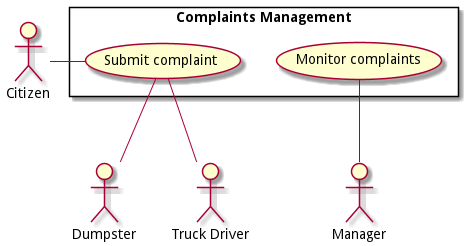
\includegraphics[width=\textwidth]{uml/complaints-use-cases.pm}
    \caption{Diagramma dei casi d'uso dello scenario della gestione dei reclami.}
    \label{fig:uml/complaints-use-cases}
\end{figure}


\begin{figure}[H]
    \centering
    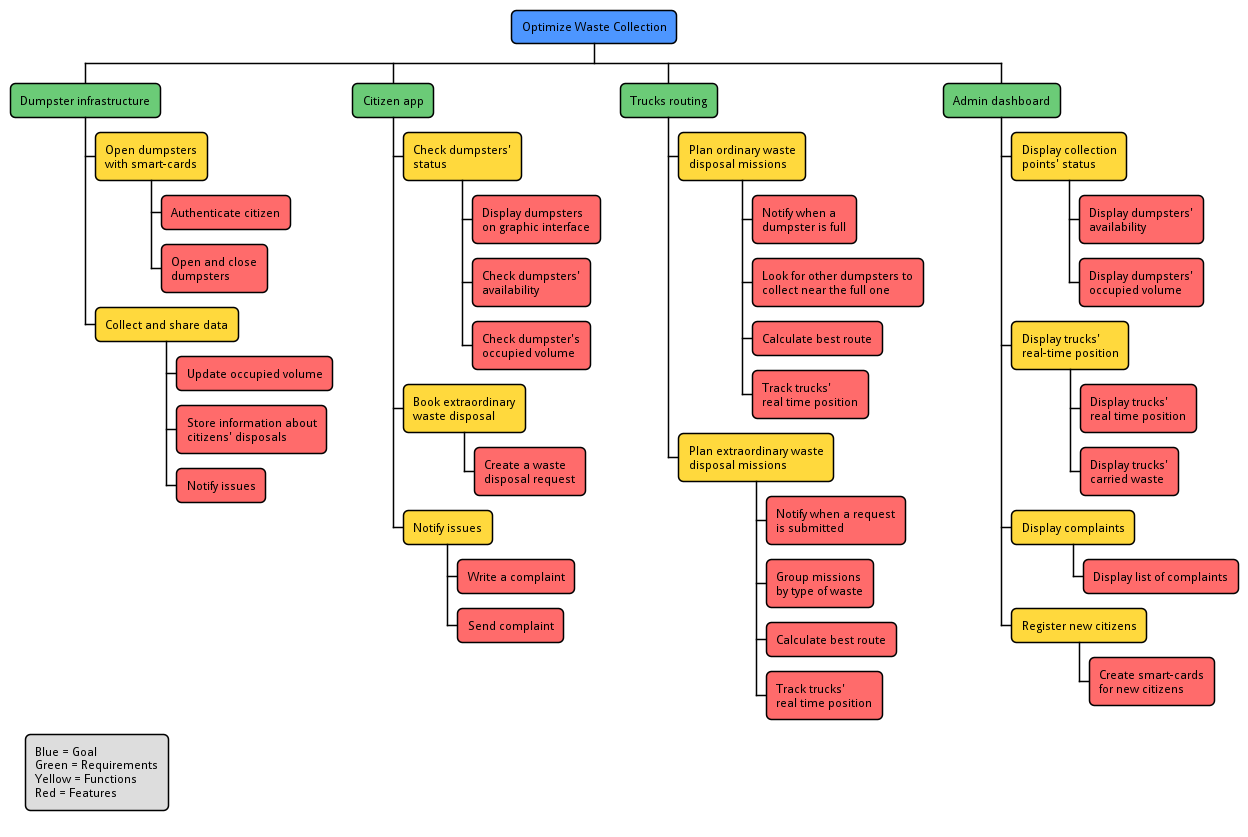
\includegraphics[width=\textwidth]{uml/requirement-breakdown-structure.pm}
    \caption{\textit{Requirement Breakdown Structure} derivata dall'analisi delle \textit{user stories} e parzialmente inclusa nel \textit{Project Overview Statement}  }
    \label{fig:uml/requirement-breakdown-structure}
\end{figure}


\begin{figure}[H]
    \centering
    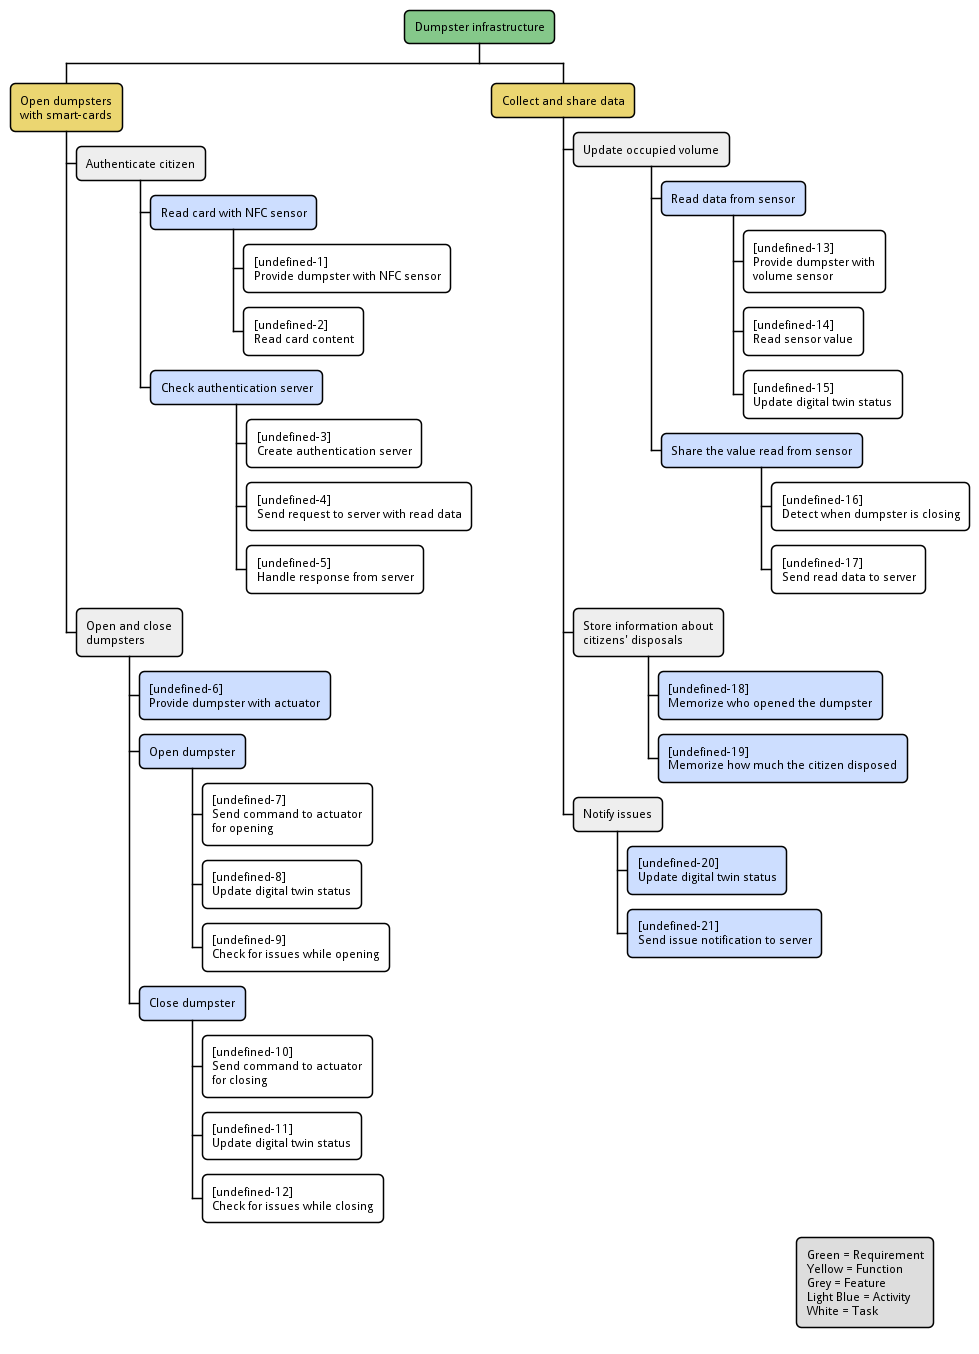
\includegraphics[width=\textwidth]{uml/wbs-dumpster-infrastructure.pm}
    \caption{\textit{Work Breakdown Structure} della \textbf{Dumpster Infrastructure}.}
    \label{fig:uml/wbs-dumpster-infrastructure}
\end{figure}


\begin{figure}[H]
    \centering
    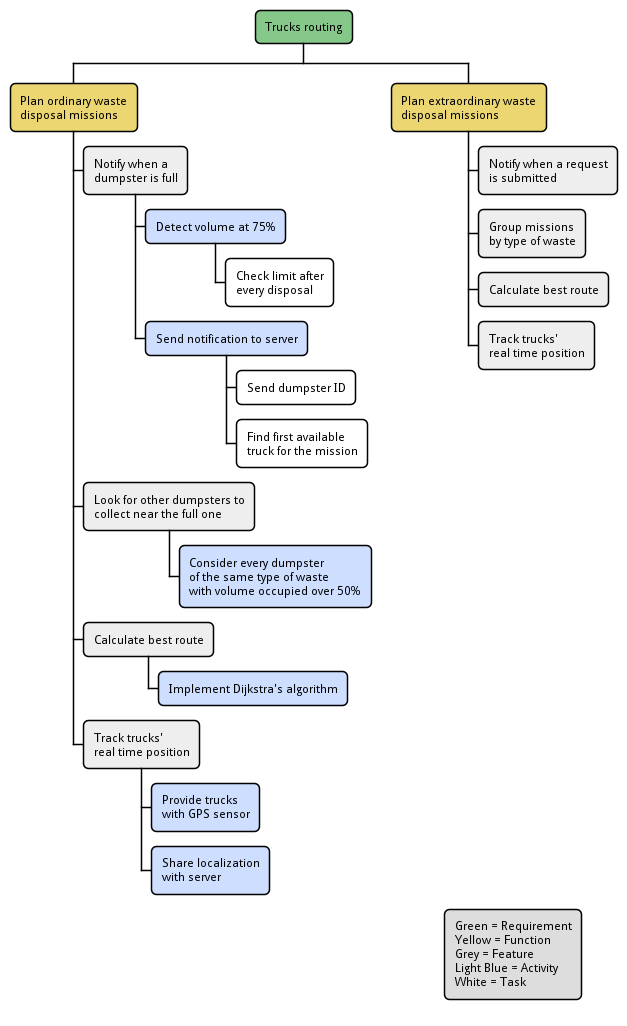
\includegraphics[width=\textwidth]{uml/wbs-trucks-routing.pm}
    \caption{\textit{Work Breakdown Structure} del \textbf{Trucks Routing}.}
    \label{fig:uml/wbs-trucks-routing}
\end{figure}


\begin{figure}[H]
    \centering
    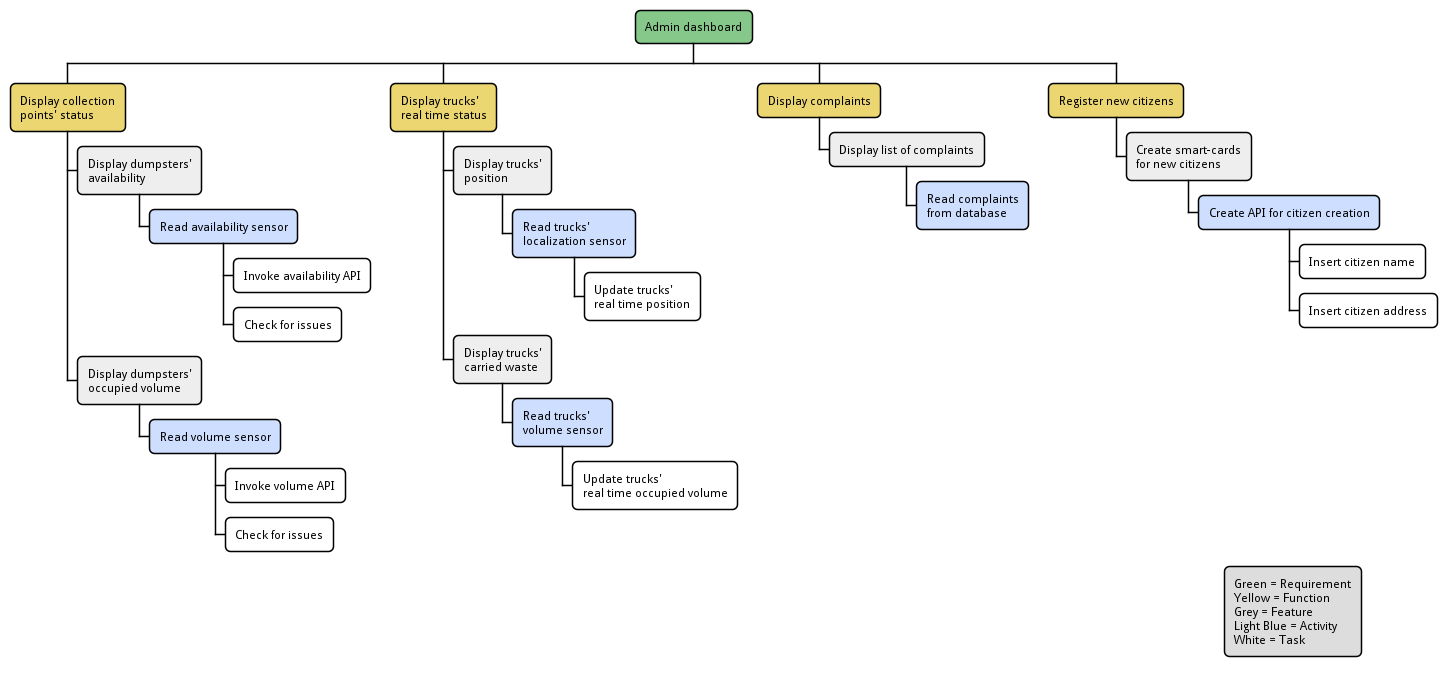
\includegraphics[width=\textwidth]{uml/wbs-admin-dashboard.pm}
    \caption{\textit{Work Breakdown Structure} della \textbf{Admin Dashboard}.}
    \label{fig:uml/wbs-admin-dashboard}
\end{figure}


\begin{figure}[H]
    \centering
    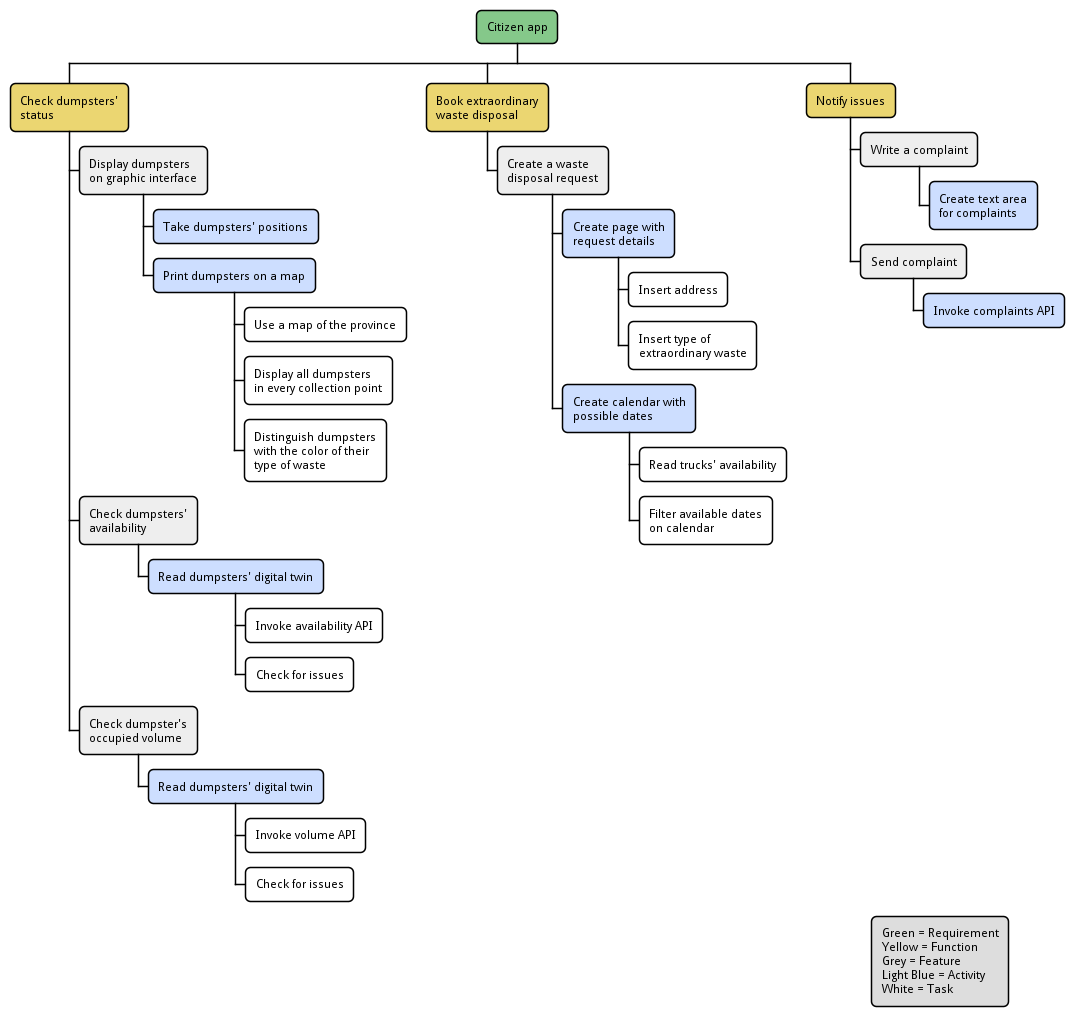
\includegraphics[width=\textwidth]{uml/wbs-citizen-app.pm}
    \caption{\textit{Work Breakdown Structure} della \textbf{Citizen App}.}
    \label{fig:uml/wbs-citizen-app}
\end{figure}

